\subchapter
{Root filesystem construction}
{Objectives:
  \begin{itemize}
  \item Explore the build output
  \item Customize the root filesystem using a {\em rootfs overlay}
  \item Customize the Linux kernel configuration
  \item Use a post-build script
  \item Customize the kernel with patches and
  \item Add more packages
  \item Use {\em defconfig} files and {\em out of tree} build
  \end{itemize}
}

\section{Explore the build output}

Now that we have discussed during the lectures the organization of the
Buildroot {\em output} tree, take some time to look inside
\code{output/} for the different build artefacts. And especially:

\begin{itemize}

\item Identify where the cross-compiler has been installed.

\item Identify where the source code for the different components has
  been extracted, and which packages have been built.

\item Identify where the target root filesystem has been created, and
  read the \code{THIS_IS_NOT_YOUR_ROOT_FILESYSTEM} file.

\item See where the \code{staging} symbolic link is pointing to.

\end{itemize}

\section{Use a {\em rootfs overlay} to setup the network}

The BeagleBone Black Wireless does not have any Ethernet interface, so
we will use Ethernet over USB to provide network connectivity between
our embedded system and the development PC. To achieve this we will
need to:

\begin{enumerate}
\item Add an init script to setup network over USB
\item Add a configuration file that configures the network interface
  with the appropriate IP address
\end{enumerate}

\subsection{Init script for USB network setup}

There are different mechanisms to configure {\em USB gadget} with
Linux: we will use the {\em gadget configfs} interface, which allows
from user-space to create USB devices providing an arbitrary set of
functionalities\footnote{See
  \url{https://elinux.org/images/e/ef/USB_Gadget_Configfs_API_0.pdf}
  for more details}.

Since the setup of such a {\em USB gadget} is not trivial, we provide
a ready-to-use shell script that we will add to the {\em init scripts}
of the Buildroot system. The script is called \code{S30usbgadget} and
is available from this lab data directory at
\code{$HOME/__SESSION_NAME__-labs/buildroot-rootfs/}.

We could copy this script directly to our SD card, but this would mean
that the next time we reflash the SD card with the root filesystem
produced by Buildroot, we would lose those changes.

In order to automate the addition of this script to the root
filesystem as part of the Buildroot build, we will use the {\bf rootfs
  overlay} mechanism. Since this {\em overlay} is specific to our
project, we will create a custom directory for our project within the
Buildroot sources: \code{board/bootlin/beagleboneblack/}.

Within this directory, create a \code{rootfs-overlay} directory, and
in \code{menuconfig}, specify
\code{board/bootlin/beagleboneblack/rootfs-overlay} as the {\em rootfs
  overlay} (option \code{BR2_ROOTFS_OVERLAY}).

Copy the \code{S30usbgadget} script to your overlay so that it is
located in
\code{board/bootlin/beagleboneblack/rootfs-overlay/etc/init.d/S30usbgadget}. At
boot time, the default init system used by Buildroot will execute all
scripts named \code{SXX*} in \code{/etc/init.d}.

\subsection{IP address configuration}

By default, Buildroot uses the \code{ifup} program from BusyBox, which
reads the \code{/etc/network/interfaces} file to configure network
interfaces. So, in \code{board/bootlin/beagleboneblack/rootfs-overlay},
create a file named \code{etc/network/interfaces} with the following
contents:

\begin{fileinput}
auto lo
iface lo inet loopback

auto usb0
iface usb0 inet static
      address 192.168.42.2
      netmask 255.255.255.0
\end{fileinput}

Then, rebuild your system by running \code{make}. Here as well, we
don't need to do a full rebuild, since the {\em rootfs overlays} are
applied at the end of each build. You can check in
\code{output/target/etc/init.d/} and \code{output/target/etc/network/}
if both the init script and network configuration files were properly
copied.

Reflash the root filesystem on the SD card, and boot your BeagleBone
Black. It should now have an IP address configured for \code{usb0} by
default.

\section{Configure the network on your host}

In the next sections of this lab, we will want to interact with the
BeagleBone Black over the network, through USB. So in this section,
we'll configure your host machine to assign an appropriate IP address
for the USB network interface.

On Ubuntu, the network interfaces corresponding to Ethernet-over-USB
connections are named \code{enx<macaddr>}. The host MAC address is
hardcoded in the \code{S30usbgadget} script to
\code{f8:dc:7a:00:00:01}, so the interface will be named
\code{enxf8dc7a000001}.

To configure an IP address for this interface on your host machine,
we'll use NetworkManager and its command line interface:

\begin{bashinput}
nmcli con add type ethernet ifname enxf8dc7a000001 ip4 192.168.42.1/24
\end{bashinput}

{\em Note: using \code{ip} in the command line is not
recommended, because Network Manager will unconfigure and
reconfigure the network interface each time the board is rebooted.}

Once this is done, make sure you can communicate with your target
using \code{ping}.

\section{Add {\em dropbear} as an SSH server}

As a first additional package to add to our system, let's add the {\em
dropbear} SSH client/server. The server will be running on the
BeagleBone Black, which will allow us to connect over the network to
the BeagleBone Black.

Run \code{make menuconfig}, and enable the \code{dropbear}
package. You can use the search capability of \code{menuconfig} by
typing \code{/}, enter \code{DROPBEAR}. It will give you a list of
results, and each result is associated with a number between
parenthesis, like \code{(1)}. Then simply press \code{1}, and
\code{menuconfig} will jump to the right option.

After leaving \code{menuconfig}, restart the build by running
\code{make}.

In this case, we do not need to do a full rebuild, because a simple
\code{make} will notice that the \code{dropbear} package has not been
built, and will therefore trigger the build process.

Re-extract the root filesystem tarball in the \code{rootfs} partition
of the SD card. Don't forget to replace the entire root filesystem:

\begin{bashinput}
rm -rf /media/$USER/rootfs/*
sudo tar -C /media/$USER/rootfs/ -xf output/images/rootfs.tar
\end{bashinput}

Now, boot the new system on the BeagleBone Black. You should see a
message:

\begin{verbatim}
Starting dropbear sshd: OK
\end{verbatim}

Now, from your PC, if you try to SSH to the board by doing:

\begin{bashinput}
ssh root@192.168.42.2
\end{bashinput}

\section{Use a post-build script}

Write a shell script that creates a file named \code{/etc/build-id} in
the root filesystem, containing the Git commit id of the Buildroot
sources, as well as the current date. Since this script will be
executed as a post-build script, remember that the first argument
passed to the script is \code{$(TARGET_DIR)}.

Register this script as a post-build script in your Buildroot
configuration, run a build, and verify that \code{/etc/build-id} is
created as expected.

\section{Patch the Linux kernel}

Now, we would like to connect an additional peripheral to our system:
the {\em Wii Nunchuk}. Using this custom peripheral requires adding a
new driver to the Linux kernel, making changes to the Device Tree
describing the hardware, and changing the kernel configuration. This
is the purpose of this section.

We will first create a new directory to store our kernel patches. It
will sit next to our {\em rootfs overlay} in our project-specific
directory:

\begin{bashinput}
mkdir board/bootlin/beagleboneblack/patches/linux/
\end{bashinput}

Copy in this directory the two patches that we provided with the data
of this lab, in \code{$HOME/__SESSION_NAME__-labs/buildroot-rootfs/linux/}:

\begin{bashinput}
cp $HOME/__SESSION_NAME__-labs/buildroot-rootfs/linux/*.patch \
     board/bootlin/beagleboneblack/patches/linux/
\end{bashinput}

The first patch adds the driver, the second patch adjusts the Device
Tree. Feel free to look at them. If you're interested, you can look at
our training course {\em Embedded Linux kernel driver development},
which precisely covers the development of this driver.

Now, we need to tell Buildroot to apply these patches before building
the kernel. To do so, run \code{menuconfig}, go the to the {\em Build
  options} menu, and adjust the \code{Global patch directories} option
to \code{board/bootlin/beagleboneblack/patches/}.

Let's now clean up completely the \code{linux} package so that its
sources will be re-extracted and our patches applied the next time we
do a build:

\begin{bashinput}
make linux-dirclean
\end{bashinput}

If you check in \code{output/build/}, the \code{linux-<version>}
directory will have disappeared.

Now, we need to adjust our kernel configuration to enable the {\em Wii
Nunchuk} driver. To start the Linux kernel configuration tool, run:

\begin{bashinput}
make linux-menuconfig
\end{bashinput}

This will:

\begin{itemize}
\item Extract the Linux kernel sources
\item Apply our two patches
\item Load the defined kernel configuration, from \code{omap2plus_defconfig}
\item Start the kernel \code{menuconfig} tool
\end{itemize}

Once in the kernel \code{menuconfig}, enable the option
\kconfig{CONFIG_JOYSTICK_WIICHUCK}, and make sure it is enabled
statically. Also, make sure the \kconfig{CONFIG_INPUT_EVDEV} option is
enabled statically (by default it is enabled as a module). Once those
options are set, leave the kernel \code{menuconfig}.

Your kernel configuration has now been customized, but those changes
are only saved in \code{output/build/linux-<version>/.config}, which
will be deleted at the next \code{make clean}. So we need to save such
changes persistently. To do so:

\begin{enumerate}

\item Run Buildroot \code{menuconfig}

\item In the \code{Kernel} menu, instead of \code{Using a defconfig},
  chose \code{Using a custom config file}. This will allow us to use
  our own custom kernel configuration file, instead of a pre-defined
  {\em defconfig} that comes with the kernel sources.

\item In the \code{Configuration file path}, enter
  \code{board/bootlin/beagleboneblack/linux.config}.

\item Exit \code{menuconfig}

\item Run \inlinebash{make linux-update-defconfig}. This will generate
  the configuration file in
  \code{board/bootlin/beagleboneblack/linux.config}. It will be a {\em
    minimal} configuration file (i.e. a {\em defconfig}). In this
  file, verify that the option \kconfig{CONFIG_JOYSTICK_WIICHUCK} is
  properly set to \code{y}.

\end{enumerate}

You can now restart the build of the kernel:

\begin{bashinput}
make
\end{bashinput}

It should hopefully end successfully, and if you look closely at the
build log, you should see the file \code{wiichuck.c} being compiled.

\section{Connect the Wii Nunchuk}

Take the nunchuk device provided by your instructor.

We will connect it to the second I2C port of the CPU (\code{i2c1}),
with pins available on the \code{P9} connector.

Identify the 4 pins of the nunchuk connector:

\begin{center}
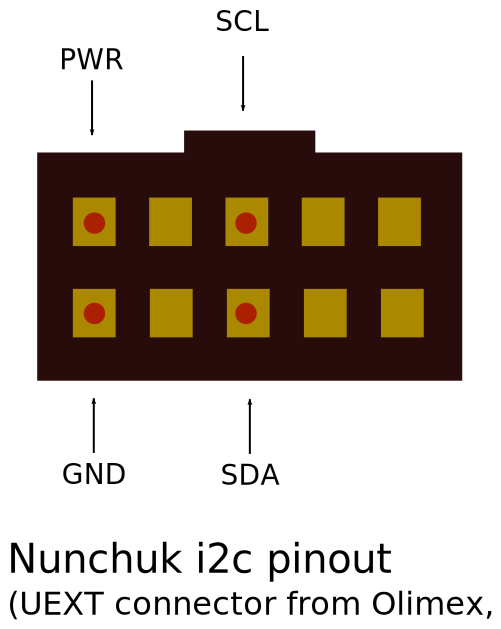
\includegraphics[width=4cm]{common/nunchuk-pinout.pdf}
\end{center}

Connect the nunchuk pins:
\begin{itemize}
\item The \code{GND} pin to P9 pins 1 or 2 (\code{GND})
\item The \code{PWR} pin to P9 pins 3 or 4 (\code{DC_3.3V})
\item The \code{CLK} pin to P9 pin 17 (\code{I2C1_SCL})
\item The \code{DATA} pin to P9 pin 18 (\code{I2C1_SDA})
\end{itemize}

\begin{center}
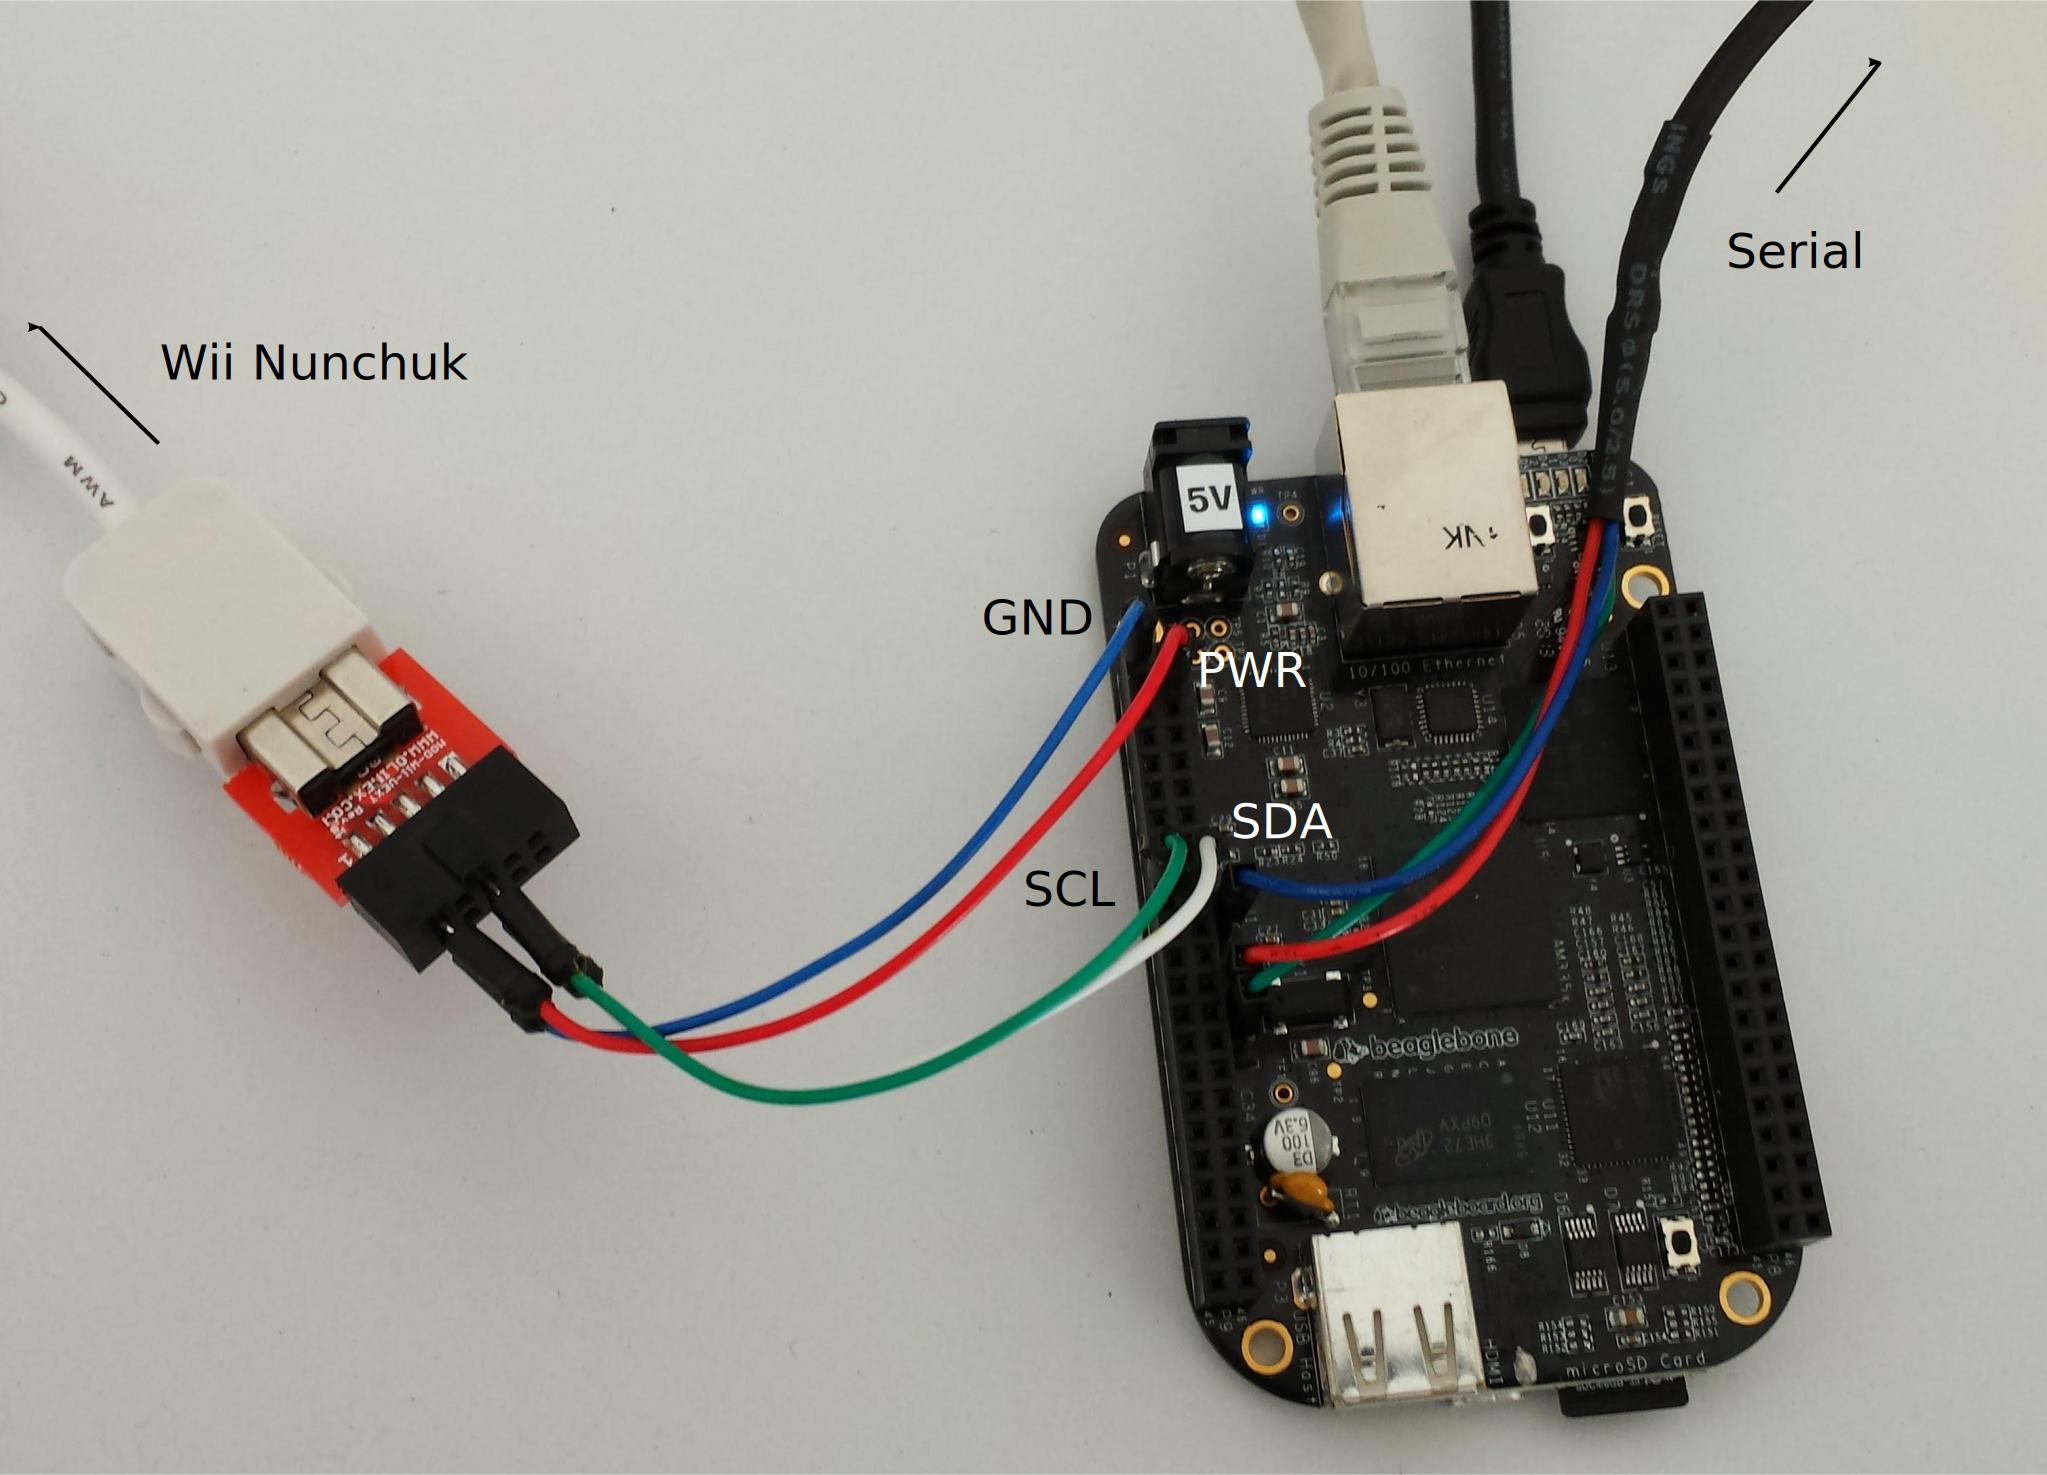
\includegraphics[width=12cm]{common/bbb-connect-nunchuk.pdf}
\end{center}

\section{Test the {\em nunchuk}}

Reflash your system, both the {\em Device Tree}, Linux kernel image
and root filesystem, and boot it.

In the kernel boot log, you should see a message like:

\begin{verbatim}
input: Wiichuck expansion connector as /devices/platform/ocp/4802a000.i2c/i2c-1/1-0052/input/input0
\end{verbatim}

You can also explore {\em sysfs}, and see that your Nunchuk device is
handled by the system:

\begin{bashinput}
cat /sys/bus/i2c/devices/1-0052/name
\end{bashinput}

Now, to get the raw events coming from the Nunchuk, you can do:

\begin{bashinput}
cat /dev/input/event0
\end{bashinput}

or, if you prefer to see hexadecimal values instead of raw binary:

\begin{bashinput}
cat /dev/input/event0 | hexdump -C
\end{bashinput}

You should see events when moving the Nunchuk (it has an
accelerometer), when moving the joystick and pushing the buttons.

\section{Add and use {\em evtest}}

Since the raw events from the Nunchuk are not very convenient to read,
let's install an application that will decode the raw input events
and display them in a more human readable format: \code{evtest}.

Enable this package in Buildroot, restart the build, reflash the root
filesystem and reboot the system. Now you can use \code{evtest}:

\begin{bashinput}
evtest /dev/input/event0
\end{bashinput}

\section{Generate a {\em defconfig}}

Now that our system is already in a good shape, let's make sure its
configuration is properly saved and cannot be lost. Go in
\code{menuconfig}, and in the \code{Build options} menu. There is an
option called \code{Location to save buildroot config} which indicates
where Buildroot will save the {\em defconfig} file generated by
\code{make savedefconfig}. Adjust this value to
\code{$(TOPDIR)/configs/bootlin_defconfig}.

Then, exit \code{menuconfig}, and run:

\begin{bashinput}
make savedefconfig
\end{bashinput}

Read the file \code{configs/bootlin_defconfig} generated in the
Buildroot sources. You will see the values for all the options for
which we selected a value different from the default. So it's a very
good summary of what our system is.

Identify the options related to the following aspects of the system:

\begin{itemize}
\item The architecture specification
\item The toolchain definition
\item The system configuration
\item The Linux kernel related configuration
\item The selection of packages
\item The U-Boot related configuration
\end{itemize}

\section{Testing a full rebuild}

To make sure that we are able to rebuild our system completely, we'll
start a build from scratch. And to learn something new, we'll use {\em
  out of tree} build.

To do so, create a build directory anywhere you want, and move inside
this directory:

\begin{bashinput}
mkdir ~/bootlin/buildroot-build/
cd ~/bootlin/buildroot-build/
\end{bashinput}

Now, we will load the \code{bootlin_defconfig}:

\begin{bashinput}
make -C ~/bootlin/buildroot/ O=$(pwd) bootlin_defconfig
\end{bashinput}

Let's explain a little bit what happens here. By using
\code{-C ~/bootlin/buildroot/}, we in fact tell \code{make} that the
\code{Makefile} to analyze is not in the current directory, but in the
directory passed as the \code{-C} argument. By passing \code{O=}, we
tell Buildroot where all the output should go: by default it goes in
\code{output/} inside the Buildroot sources, but here we override that
with the current directory (\code{$(pwd)}).

This command will have two main effects:

\begin{enumerate}

\item It will load the \code{bootlin_defconfig} as the current
  configuration. After running the command, read the file named
  \code{.config}. It's much longer than the {\em defconfig}, because
  it contains the values for all options.

\item It will create a minimal \code{Makefile} in this output
  directory, which will allow us to avoid doing the \code{make -C
    ... O=...} dance each time.

\end{enumerate}

Now that this is done, start the build. You can again save the build
log:

\begin{bashinput}
make 2>&1 | tee build.log
\end{bashinput}
